\newenvironment{mytest}[4]
{
    \begin{center}
        \centering
        \begin{tabular}[h]{|m{4cm}|m{12cm}|} 
            \hline
            \rowcolor[HTML]{F8B400}
            \textbf{But} & #1 \\
            \hline
            \hline
            \rowcolor[HTML]{F7F7F7}
            Entrée & #2 \\
            \hline
            \rowcolor[HTML]{F7F7F7}
            Scénario & #3 \\
            \hline
            \rowcolor[HTML]{F7F7F7}
            Analyse du test & #4 \\
            \hline
        \end{tabular}
    \end{center}  
}

\section{Nos tests}

Nous avons mis en place divers outils pour contrôler notre implémentation :
\begin{itemize}
    \item Chaque \emph{commit} sera vérifier par des pipelines de \emph{GitLab}. Cet outil compile le code proposé sur une machine afin de voir si le code suggérer n'a aucune erreur de compilation.
    \item L'implémentation de notre \emph{backend} est contrôlé par le framework \emph{NYC}. Nos tests sont surveillés par le framework et nous donne le résultat de \emph{coverage} pour chaque fichier testé.
\end{itemize}

\subsection{Test unitaire}

Consigne : description des tests, discussion de leurs résultats, explication des problèmes, des défauts et bugs. Pour chacun des tests avec : (1) spécification et buts du test ;
(2) cas de tests (données) utilisé ; (3) scénario du test ; (4) analyse du test et les moyens de mise en œuvre de cette analyse.

\subsubsection{Vérification des fichiers dans le fichier \emph{src}}

\mytest
{Vérifier si les fichiers possède le bon format (\texttt{.ts}) dans le dossier \texttt{src/main}}
{Un ensemble de fichiers}
{En cas de mauvais format dans le dossier, on affiche les fichiers qui ne respectent pas le format \texttt{.ts}}
{Parcours d'un dossier en ajoutant dans une liste les fichiers qui ne respecte pas la condition}

\mytest
{Vérifier si les fichiers possède le bon format (\texttt{.ts} ou \texttt{.json}) dans le dossier \texttt{src/test}}
{Un ensemble de fichiers}
{En cas de mauvais format dans le dossier, on affiche les fichiers qui ne respectent pas le format \texttt{.ts} ou \texttt{.json}}
{Parcours d'un dossier en ajoutant dans une liste les fichiers qui ne respecte pas la condition}

\mytest
{Chaque fichier possède une classe doit commencer par une majuscule dans le dossier \texttt{src/main}}
{Un ensemble de fichiers}
{En cas de non-respect des consignes, on affiche les fichiers qui ne respectent la capitalisation de la première lettre}
{On ajoute dans une liste les fichiers qui ne respecte pas la condition (parcours d'un dossier + manipulation de chaîne de caractère pour récupérer la première}

\subsubsection{Vérification de la carte du jeu}

\mytest
{Vérification de l'emplacement d'une case d'hexagone \#1}
{Identifiant d'une vraie case d'hexagone}
{Si l'identifiant n'est pas sur la carte du jeu, signalez cette case}
{Vérifie l'identifiant dans une table de hachage}

\mytest
{Vérification de l'emplacement d'une case d'hexagone \#2}
{Identifiant d'une fausse case d'hexagone}
{Si l'identifiant est inclus sur la carte du jeu, signalez cette case}
{Vérifie l'identifiant dans une table de hachage}

\subsubsection{Vérification du serveur socket}

TODO

\subsubsection{Vérification de l'instance de la machine d'état}

TODO

\subsubsection{Vérification de la machine d'état}

TODO

\subsubsection{Vérification de l'instance du jeu}

TODO

\subsubsection{Vérification de joueur}

TODO

\subsubsection{Vérification de la classe abstraite \emph{Player}}

TODO

\subsubsection{Vérification d'une base}

TODO

\subsubsection{Vérification des bases}

TODO

\subsubsection{Vérification de l'attaque}

\mytest
{Vérifier si le combat retourne les bons résultats de dégats et applique les bons effets}
{Une unité attaquante et une unité defenseuse}
{Si un résultat doit détruire une unité ou au contraire ne rien faire, les effets se repercutent dans le jeu}
{Nous verifions pour les résultats aleatoires possibles, tout résultat de combat est bien appliqué. Nottament vérifier
que une unité est bien détruite, si elle perd les bons points de vie ou si elle est toujours vivante}

\mytest
{Vérifier si le combat retourne les bons résultats de morale et applique les bons effets}
{Une unité attaquante et une unité defenseuse}
{Si un résultat doit forcer une unité à se replier ou non, alors le changement doit être visible dans le jeu}
{Nous verifions pour les résultats aleatoires possibles, que si une unité doit se replier, alors l'unité se
deplace loin de l'ennemie. Si il faut pas alors elle doit rester au même endroit.}

\subsubsection{Vérification du combat}

\mytest
{Vérifier si le simulateur de combat retourne les bons résultats pour les degats}
{Un nombre d'attaquants et de defenseurs, un entier représentant le morale et un type de terrain}
{Chaque combinaison de paramètres doit retourner le même résultat exact à chaque fois}
{Nous prenons quatres combinaisons d'entrées distinctes. 
En divisant le nombre d'attaquants par le nombre de défenseurs, on applique les règles du jeu pour definir
quelle case du tableau des résultats de combat il faut obtenir. Pour ne pas avoir des résultats aleatoires comme
il le faut normalement et avoir des tests exacts, nous ne lancons pas de dé.}

\mytest
{Vérifier si le simulateur de combat retourne les bons résultats pour le morale}
{Un nombre d'attaquants et de defenseurs, un entier représentant le morale et un type de terrain}
{Chaque combinaison de paramètres doit retourner le même résultat exact à chaque fois}
{Nous prenons les même quatres combinaisons d'entrées distinctes. 
En divisant le nombre d'attaquants par le nombre de défenseurs, on applique les règles du jeu pour definir
quelle case du tableau des résultats de combat il faut obtenir. Pour ne pas avoir des résultats aleatoires comme
il le faut normalement et avoir des tests exacts, nous ne lancons pas de dé.}


\subsubsection{Vérification du jeu}

TODO

\subsubsection{Vérification de la recherche du plus court chemin}

\mytest
{Vérifier si le chemin renvoyé est le plus court}
{Identifiant d'un hexagone de départ, l'identifiant d'un hexagone de destination et l'unité qui se deplace}
{Pour un hexagone de départ et de destination donné, un plus court chemin a toujours le même poids. Nous verifions
si il est égale à celui ci}
{En ayant une unité qui est adjacente à une unité ennemie, nous verifions si le calcul de cout est correcte, car
le plus court chemin passe à coté d'elle, ce qui teste plusieurs scenarios qui peuvent être rencontrés dans le jeu}

\mytest
{Vérifier si une unité ne passe pas par un hexagone qui contient des ennemis}
{Identifiant d'un hexagone de départ, l'identifiant d'un hexagone de destination et l'unité qui se deplace}
{Si on trouve un plus court chemin entre deux hexagones, le chemin ne doit pas contenir un hexagone qui a des
unités ennemies.}
{En prenant un plus court chemin, nous verifions pour tout les hexagones du chemin, si il n'appartient pas
au joueur qui tente de bouger l'unité.}

\subsection{Couverture du code}

Le framework \emph{NYC} nous permet de tester la couverture. Il faut lancer la commande \emph{yarn test} dans le \lstinline{backend} ce qui créé dans le dossier \lstinline{coverage} où se trouve à l'intérieur un \lstinline{index.html} qui donne ceci.

\begin{figure}[H]
    \centering
    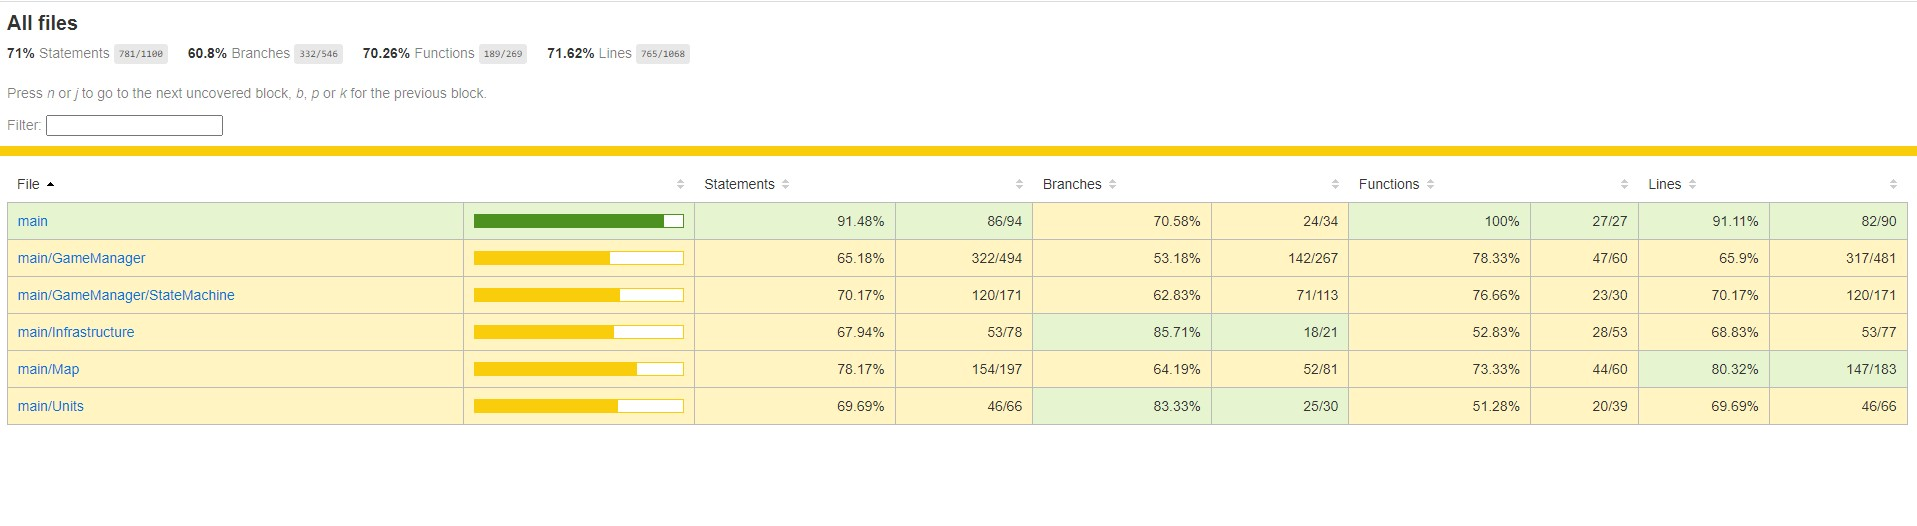
\includegraphics[scale=0.35]{data/couverture_test_1.jpg}
    \caption{Couverture générale du backend}
\end{figure}

On peut voir le pourcentage de couverture de chaque fichier. On peut aussi aller plus dans les détails et regarder ligne par ligne pour être sûr qu'absolument tout le code soit testé.

\begin{figure}[H]
    \centering
    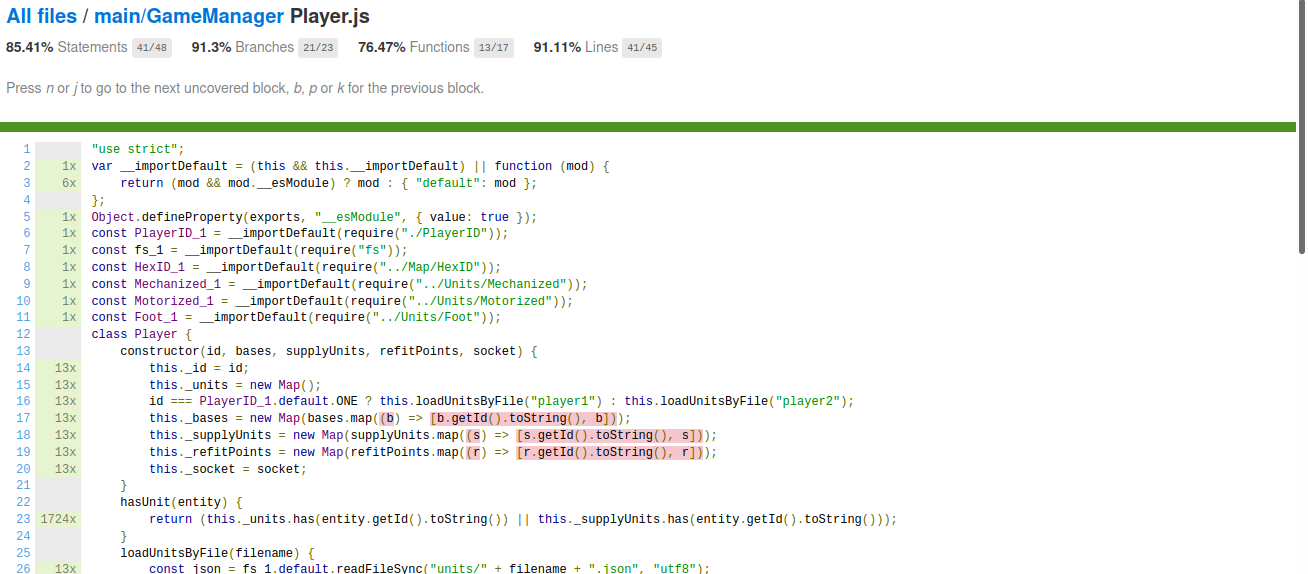
\includegraphics[scale=0.3]{data/couverture_test_2.png}
    \caption{Couverture d'un fichier}
\end{figure}

La couverture du code n'implique pas des tests de qualité. Après quelques recherches nous avons trouvé qu'une couverture minimale de bonne qualité dépasse les 80\%. Nous nous sommes donc fixés d'au moins atteindre ce pourcentage.